\documentclass{sciposter}
\usepackage{lipsum}
\usepackage{listings}
\usepackage{epsfig}
\usepackage[dvipsnames]{xcolor}
\usepackage{amsmath}
\usepackage{amssymb}
\usepackage{multicol}
\usepackage{graphicx,url}
\usepackage[portuges, brazil]{babel}   
\usepackage[utf8]{inputenc}

\newtheorem{Def}{Definition}


\title{\Huge \texttt{{\color{NavyBlue}XI SEMANA UNIFICADA DE APRESENTAÇÕES}}}

\author{Caroline B. do E. Santo, Mahaira S. de Souza, Thiago de S. Messias}

\institute{\texttt{{\bf{\color{orange} 8 a 12 de Junho de 2015\\
Bacharelado em Ciência da Computação – Código: BCC\_PI\_III\_N\_G01}}}}

\leftlogo[1]{Senac-logo}


\begin{document}

\conference{{\bf PI III}- Senac, 25 de Maio de 2015, São Paulo, Brasil}

\maketitle

{\center

{\bf { \huge  Projeto Integrador III - Sistema Autônomo - AirDrums} } 

}


\bf{\hrulefill}
\begin{multicols}{3}

\section {Resumo}
De acordo com o proposto na disciplina Projeto Integrador III, a partir do estudo e aplicação de algoritmos relacionados a visão computacional, indiretamente através da biblioteca multiplataforma OPENCV[1], foi desenvolvido o AirDrums, uma bateria em forma de jogo, onde o jogador deve seguir uma sequência de passos para tocar a música e passar de fase, para isso, foi utilizada a biblioteca gráfica  allegro 5[2] e a linguagem de programação C-99[3]. HSV e Ponto Médio foram os principais algoritmos para obter os resultados desejados.

\section{Introducão}
AirDrums é um jogo, cujo o objetivo é acertar os alvos que caem em cascata para arrematar pontos ao final da música, onde a interação do jogador ocorre via duas baquetas com pontas coloridas (azul e vermelho), detectavél via algoritmo do HSV.
Atualmente, é comum visualizar pessoas tocando instrumentos musicais no ar, esta prática é conhecida como Air (nome do instrumento musical), desta forma originou-se o jogo, onde o intuito é proporcionar diversão de forma rápida e fácil, via visão computacional, ou seja, não é necessário a compra de uma bateria, o jogador pode utilizar uma caneta, lápis, baquetas e etc, desde que os objetivos condizam com as cores propostas. 

\begin{figure}[!htb]
\centering

\includegraphics[width=20cm]{lapisV.jpg}
\caption{Imagem ilustrativa Lápis/Baquetas}
\label{baquetas}
\end{figure}


\section{Desenvolvimento}

Conforme proposto pelo escopo do Projeto Interativo III - Sistema Autômato, foi desenvolvido o jogo AirDrums, utilizando linguagem C - versão 99, usando a biblioteca Allegro5 e OpenCV. \\

\textbf{\subsection{Detecção de cores}}
AirDrums rastreia as cores localizadas na ponta das duas baquetas nas cores azul e vermelho. Para tal resultado o HSV[4] foi indispensável.
\textit{\textbf{\subsubsection{HSV: O que é, e como funciona:}}} \\
HSV é a abreviação para Hue (Matriz), Saturation (Saturação), e value (Valor). A matriz define o tipo de cor, que pode variar entre $0\,^{\circ}$, e $360\,^{\circ}$. A saturação é a pureza da imagem, que quanto mais próxima de 0\% mais escura será, e quanto mais próximo de 100\% mais pura será. O valor define o brilho da imagem possibilitando o rastreamento do objeto ignorando a  iluminação do ambiente, e assim como a saturação  de 0\% á 100\%. \\

A imagem abaixo mostra como este sistema de cores funciona:

\begin{figure}[!htb]
\centering
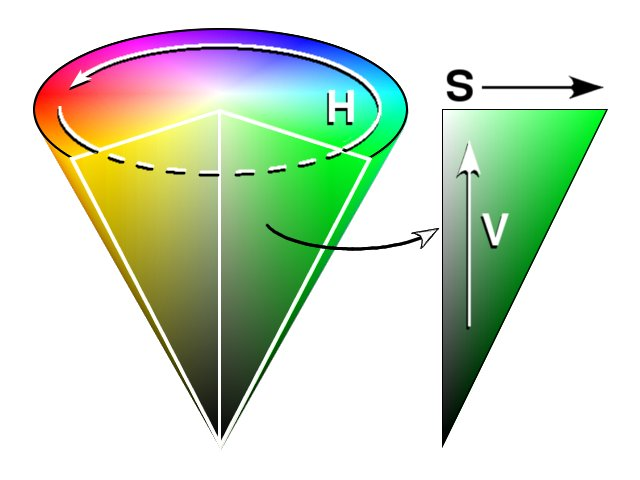
\includegraphics[scale=0.6]{HSV_cone.jpg}
\caption{Exemplo: HSV}
\end{figure}

\subsection{Música}

Cada trecho da música equivale a uma matriz 4x4, desta forma o alvo aparece na posição da matriz com o elemento "1", ignorando o elemento "0", assim como mostra o exemplo abaixo
\\
\\

$ Exemplo =\left[\begin{array}{rrrr}
0 & 0 & 0 & 0\\
0 & 0 & 1 & 0\\
0 & 1 & 0 & 1\\
1 & 0 & 0 & 0
\end{array}\right],\quad$

\begin{figure}[!htb]
\centering
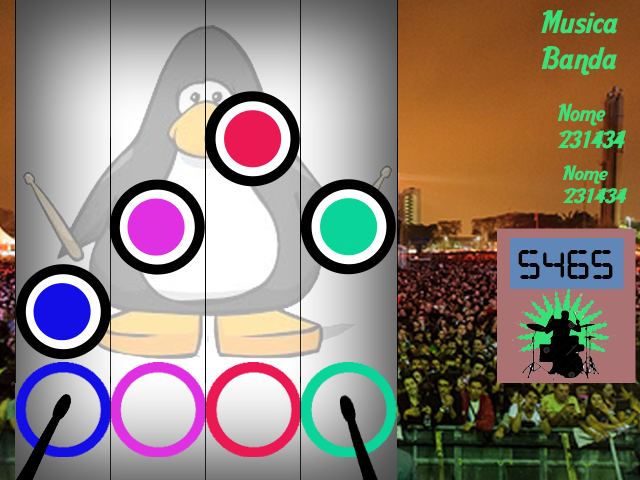
\includegraphics[width=20cm]{Exemple.png}
\caption{Alvos com posições de acordo com a matriz}
\label{alvos}
\end{figure}

\subsection{Centróide}

\textbf{Ponto médio} é o centro geométrico, ou seja o centro da massa. No jogo ele calcula o valor médio da ponta das baquetas:

Ponto médio Y =  \frac{\int Y .dA \over \int dA}\\	

\\\\\\

Ponto médio X = 
\frac{\int X .dA \over \int dA} \\

Este cálculo é feito para que seja possível verificar o movimento que o jogador estará executando.

\begin{figure}[!htb]
\centering
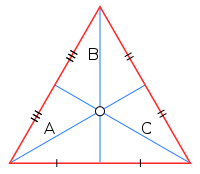
\includegraphics[width=15cm]{triangulo_cent.png}
\caption{O círculo no meio representa o ponto médio}
\end{figure}

\section{Resultados }

Evolução do jogo, no quesito telas e dificuldades do jogador: \\

Ao acertar o alvo, ele ficará preenchido com a cor correspondente ao alvo. Assim como na imagem abaixo: 

\begin{figure}[!htb]
\centering
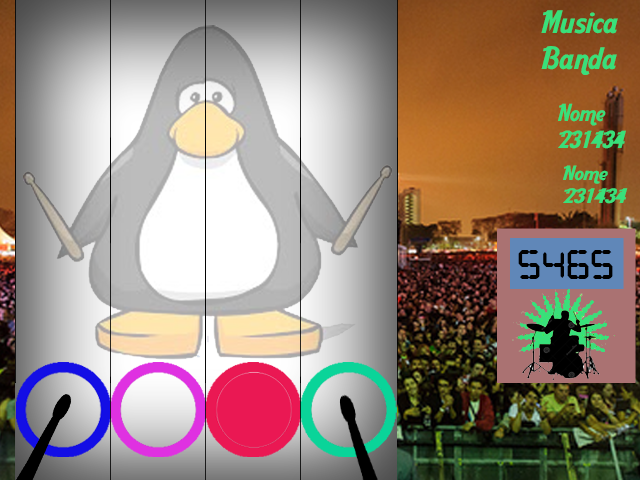
\includegraphics[scale=2.3]{AccertCase.png}
\caption{Exemplo: Caso acerto do jogador ao alvo}
\end{figure}

No entanto, se o jogador não conseguir ser rápido o suficiente para acertar o alvo, ao invés de ser preenchido com a cor correspondente, aparecerá uma caveira. Deste modo, o jogador saberá que está perdendo pontos, como mostra a imagem abaixo:

\begin{figure}[!htb]
\centering
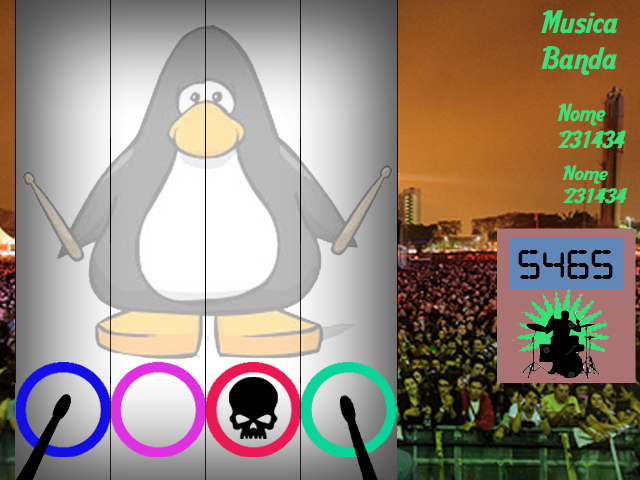
\includegraphics[scale=2.3]{ErrorCase.png}
\caption{Exemplo: Erro de alvo}
\end{figure}

Quando o jogador movimentar as baquetas, elas estarão sendo rastreadas e o cursor irá se mover de acordo com elas.

\begin{figure}[!htb]
\centering
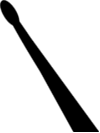
\includegraphics[scale=4.3]{cursor_right.png}
\caption{cursor}
\end{figure}

A imagem abaixo mostra menor dificuldade, pois existem menos alvos simultaneos caindo em cascata.

\begin{figure}[!htb]
\centering
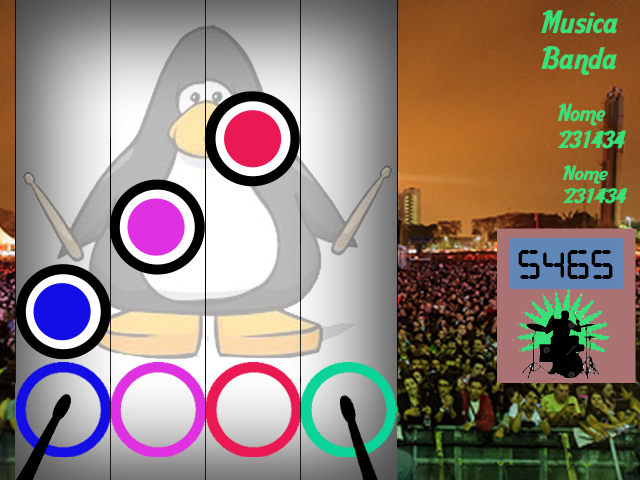
\includegraphics[scale=2.3]{easy.png}
\caption{Exemplo: Nível Facil}
\end{figure}

\section{Considerações Finais}
Levando-se em conta o que foi observado, e obtido como resultado ao decorrer do projeto, é possível afirmar que a iluminação é o fator que mais dificulta o desenvolvimento de detecção de objetos, isto requeriu algumas calibragens até chegar ao resultado desejado. 

\bibliographystyle{plain}
\begin{thebibliography}{7}

\bibitem {site OpenCV}
http://opencv.org/ \\
\newblock {OpenCV}

\bibitem {site allegro} http://www.rafaeltoledo.net/tutoriais-allegro-5/ \\
\newblock {Allegro 5.}

\bibitem {livro}
H. M. Deitel e P. J. Deitel.
\newblock {Como programar em C, 2º edição.}

\bibitem *http://sidigicor.blogspot.com.br/2011/02/modelo-hsv.html \\
\newblock {Explicação do Sistema de Cores HSV}


\end{thebibliography}

\end{multicols}
\end{document}